\documentclass[signals,article,submit,pdftex,moreauthors]{Definitions/mdpi} 

\firstpage{1} 
\makeatletter 
\setcounter{page}{\@firstpage} 
\makeatother
\pubvolume{1}
\issuenum{1}
\articlenumber{0}
\pubyear{2025}
\copyrightyear{2025}
%\externaleditor{Firstname Lastname} % More than 1 editor, please add `` and '' before the last editor name
\datereceived{ } 
\daterevised{ } % Comment out if no revised date
\dateaccepted{ } 
\datepublished{ } 
%\datecorrected{} % For corrected papers: "Corrected: XXX" date in the original paper.
%\dateretracted{} % For retracted papers: "Retracted: XXX" date in the original paper.
\hreflink{https://doi.org/} % If needed use \linebreak
%\doinum{}
%\pdfoutput=1 % Uncommented for upload to arXiv.org
%\CorrStatement{yes}  % For updates
%\longauthorlist{yes} % For many authors that exceed the left citation part

%=================================================================
% Add packages and commands here. The following packages are loaded in our class file: fontenc, inputenc, calc, indentfirst, fancyhdr, graphicx, epstopdf, lastpage, ifthen, float, amsmath, amssymb, lineno, setspace, enumitem, mathpazo, booktabs, titlesec, etoolbox, tabto, xcolor, colortbl, soul, multirow, microtype, tikz, totcount, changepage, attrib, upgreek, array, tabularx, pbox, ragged2e, tocloft, marginnote, marginfix, enotez, amsthm, natbib, hyperref, cleveref, scrextend, url, geometry, newfloat, caption, draftwatermark, seqsplit
% cleveref: load \crefname definitions after \begin{document}

%=================================================================
% Please use the following mathematics environments: Theorem, Lemma, Corollary, Proposition, Characterization, Property, Problem, Example, ExamplesandDefinitions, Hypothesis, Remark, Definition, Notation, Assumption
%% For proofs, please use the proof environment (the amsthm package is loaded by the MDPI class).

%=================================================================
% Full title of the paper (Capitalized)
\Title{Analyzing shortwave propagation with a remote accessible software defined ham radio system}

% MDPI internal command: Title for citation in the left column
\TitleCitation{Analyzing shortwave propagation with a remote accessible software defined ham radio system}

% Author Orchid ID: enter ID or remove command
\newcommand{\orcidauthorA}{0000-0000-0000-000X} % Add \orcidA{} behind the author's name
%\newcommand{\orcidauthorB}{0000-0000-0000-000X} % Add \orcidB{} behind the author's name

% Authors, for the paper (add full first names)
\Author{Gergely Vakulya $^{1}$, Firstname Lastname $^{2}$ and Gyula Simon $^{2,}$*}

%\longauthorlist{yes}

% MDPI internal command: Authors, for metadata in PDF
\AuthorNames{Firstname Lastname, Firstname Lastname and Firstname Lastname}

% MDPI internal command: Authors, for citation in the left column, only choose below one of them according to the journal style
% If this is a Chicago style journal 
% (arts, genealogy, histories, humanities, jintelligence, laws, literature, religions, risks, socsci): 
% Lastname, Firstname, Firstname Lastname, and Firstname Lastname.

% If this is a APA style journal 
% (admsci, behavsci, businesses, econometrics, economies, education, ejihpe, games, humans, ijfs, journalmedia, jrfm, languages, psycholint, publications, tourismhosp, youth): 
% Lastname, F., Lastname, F., \& Lastname, F.

% If this is a ACS style journal (Except for the above Chicago and APA journals, all others are in the ACS format): 
% Lastname, F.; Lastname, F.; Lastname, F.
\isAPAStyle{%
       \AuthorCitation{Lastname, F., Lastname, F., \& Lastname, F.}
         }{%
        \isChicagoStyle{%
        \AuthorCitation{Lastname, Firstname, Firstname Lastname, and Firstname Lastname.}
        }{
        \AuthorCitation{Lastname, F.; Lastname, F.; Lastname, F.}
        }
}

% Affiliations / Addresses (Add [1] after \address if there is only one affiliation.)
\address{%
$^{1}$ \quad Affiliation 1; e-mail@e-mail.com\\
$^{2}$ \quad Affiliation 2; e-mail@e-mail.com}

% Contact information of the corresponding author
\corres{Correspondence: e-mail@e-mail.com; Tel.: (optional; include country code; if there are multiple corresponding authors, add author initials) +xx-xxxx-xxx-xxxx (F.L.)}

% Current address and/or shared authorship
%\firstnote{Current address: Affiliation.}  
% Current address should not be the same as any items in the Affiliation section.

%\secondnote{These authors contributed equally to this work.}
% The commands \thirdnote{} till \eighthnote{} are available for further notes.

%\conference{} % An extended version of a conference paper

% Abstract (Do not insert blank lines, i.e. \\) 
\abstract{Ham radio has long been a foundational area of practice in electrical
  engineering. Advances in signal processing, particularly the advent of
  software-defined radio (SDR), have revolutionized the field, offering new
  possibilities and modes of operation. This paper introduces a system designed
  for long-term collection of shortwave propagation data, leveraging SDR
  technology. It also presents the analysis of the collected data,
  demonstrating the system's potential for advancing research in radio wave
  propagation.}

\keyword{software defined radio; shortwave propagation; data analysis; big data}



\begin{document}

\section{Introduction}

Amateur radio, commonly known as ''ham radio'' offers a diverse range of
applications and goals for enthusiasts. However, regulatory authorities and
experts emphasize one critical objective: the study of radio wave propagation.
Propagation research through amateur radio plays a vital role in understanding
how radio signals travel, interact with the atmosphere, and behave under
various conditions.

The basic element of ham radio operation is the contact, in which the mandatory
parts are the exchange of the callsigns and the signal reports. Signal report
is the characterization of the received signal, which can contain the signal strength
and other properties (signal purity, modulation quality, signal fluctuation etc.).
This information provides valuable data for studying the varying properties of radio
wave propagation.
Ham radio operators employ various modulation modes to facilitate voice, Morse
code, and data communication. In recent years, data-based contacts have gained
significant popularity, largely due to advancements in digital technology, such
as computers, sound cards, and specialized software. These highly efficient
digital modes have revolutionized ham radio by offering enhanced performance in
low-signal environments and expanding the possibilities for real-time
propagation studies.

FT8, or Franke-Taylor design, 8-Frequency Shift Keying, is a digital
communication mode developed in 2017 by Joe Taylor (K1JT) and Steven Franke
(K9AN). It has rapidly gained popularity within the amateur radio community due
to its exceptional efficiency, especially in low-power and noisy environments.
One of FT8's key features is its ability to perform automated,
computer-assisted communications, allowing for rapid exchanges of minimal data,
including callsigns, signal reports, and geo-locations, which makes it an
ideal tool for propagation research.

\section{Architecture}

\subsection{The FT8 protocol}


%FT8 is based on a 8-FSK modulation with
%
%FT8 utilizes small bandwidth (50 Hz) and transmits in 15-second synchronized intervals,
%enabling operators to make reliable contacts even with weak signals, often
%below the noise floor.

The FT8 protocol \cite{franke2020} allows for two participants to exchange their callsigns, their geolocations
and the received signal to noise ratios in a compact form. Callsigns can consist of letters
and numbers with some rules and restrictions. Special prefixes or suffixes with a / (slash)
symbol can extend the callsign in some cases.

The geolocation is encoded in 4 letter Maidenhead format, which is represented as two letters and
two digits. Each combination defines a rectangle of 2 degrees (longitude) by 1 degre (latitude).

The Signal-to-Noise Ratio (SNR) is expressed on a dB scale from -30 to +32 dB. To reduce
the number of required bits only even numbers are used.

An FT8 contact between the station of Alice (with callsign AL1CE) and the station
of Bob (with the callsign B0BB) consists of the following messages:

\begin{enumerate}

  \item{CQ AL1CE JN87}    %1

  \item{AL1CE B0BB IO83}  %2

  \item{B0BB AL1CE -15}   %3

  \item{AL1CE B0BB R-17}  %4

  \item{B0BB AL1CE RRR}   %5

  \item{AL1CE B0BB 73}    %6

  \item{B0BB AL1CE RR73}  %7
  

\end{enumerate}

Message type 1 is a general call (CQ) from Alice, which means, she is ready to
make contacts. JN87 is the Maidenhead grid square of Alice. Note that an optional designator can be applied between the CQ and the callsign,
marking a target area or a special event.

Bob can answer this with message type 2. This message contains the callsign of both stations and the grid square of Bob.

Then Alice can reply with message type 3. This message type contains the two callsigns and the signal report from Alice (-15 dB).

Message type 4 contains the callsigns, the signal report from Bob (-17 dB) and an acknowledgement for the previous message
(R, short for roger).

Then Alice acknowledges the contact with message type 5 (RRR, short for roger, roger, roger).

Message type 6 makes the contact complete, where the participants say goodbye with 73 (meaning Best Regards). An alternative
shorter version for types 5 and 6 is message type 7 (RR73).

Each message is represented as a 77-bit packet, then with Cyclic Recundancy Check (CRC) and Forward Error Coding (FEC) a 174 bit
codeword is generated. Codewords are transmitted using 8-tone CPFSK (Continuos Phase Frequency Shift Keying) with 6.25 Hz tone separation
and 6.25 symbols / sec. One FT8 message takes approx. 50 Hz bandwidth, therefore a usual 2800 Hz ham radio SSB voice channel can handle
56 parallel communications. Note that decoding of partially overlapping messages are even possible.
Unlike conventional voice communication, which requires separate frequencies for each transmission to prevent interference,
FT8 operates on a single, fixed frequency within each ham radio band, enabling multiple simultaneous communications
and data collection through passive listening and decoding.

\subsection{Hardware architecture}

\begin{figure}[htbp]
	\centering
	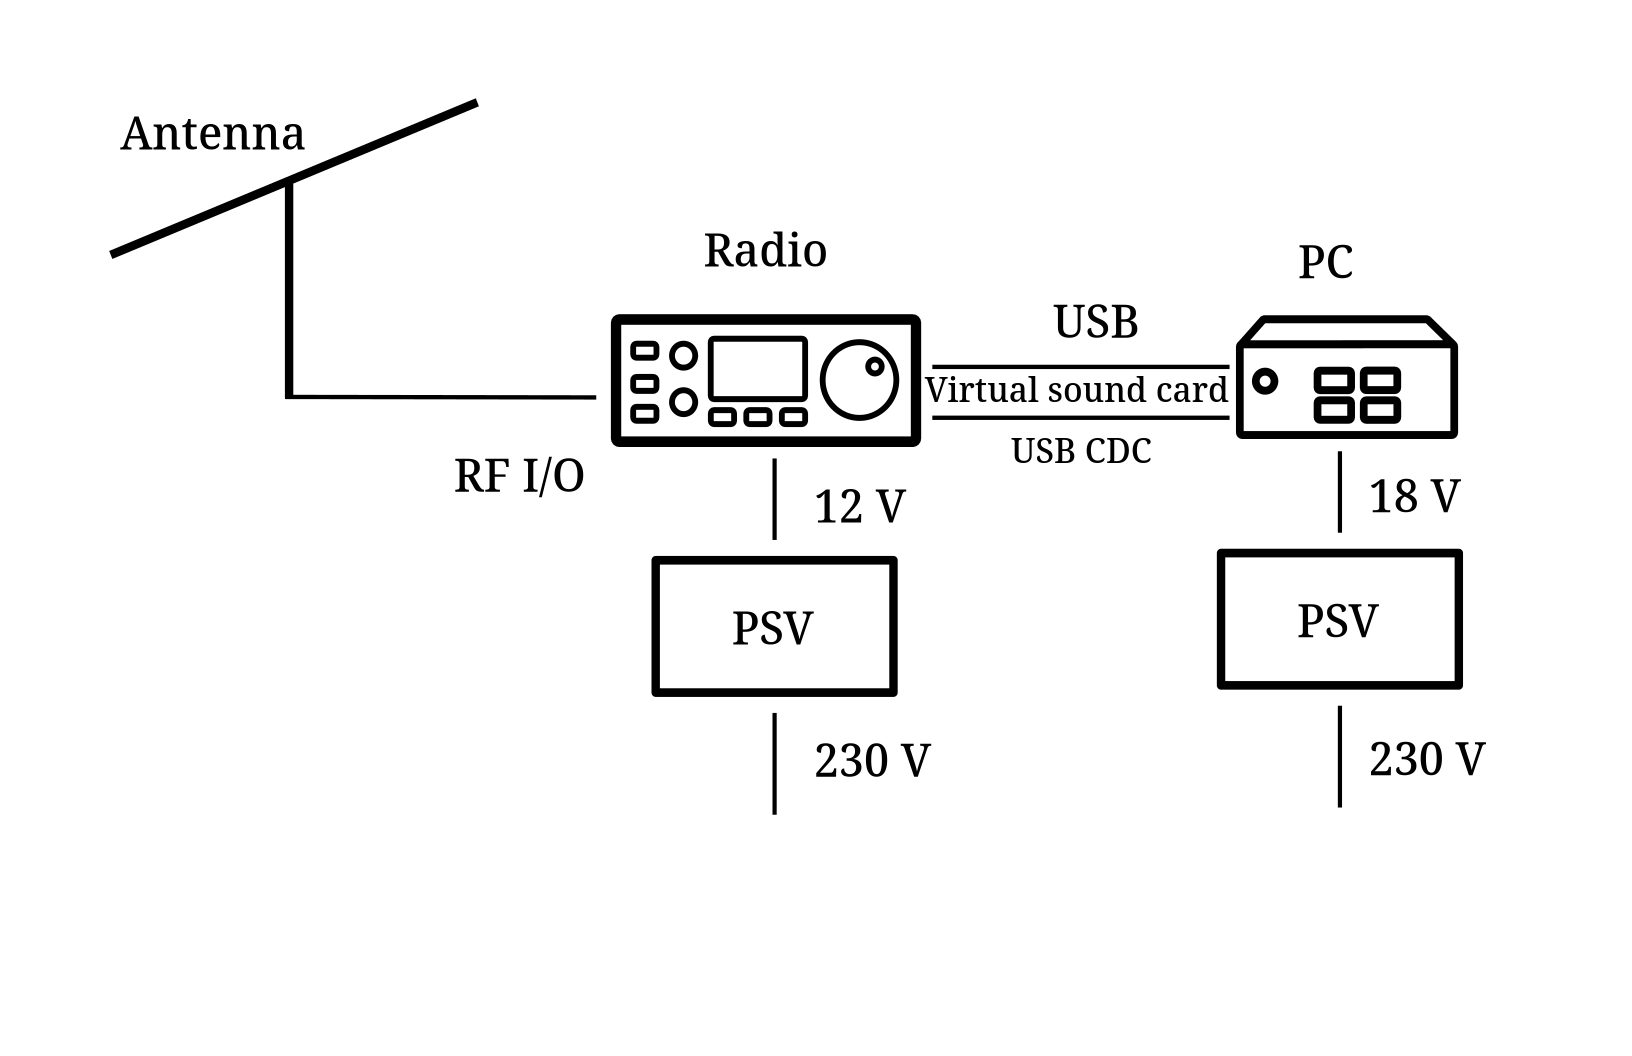
\includegraphics[width=.8\textwidth]{fig/hardware.png}
	\caption{The hardware architecture of the system}
	\label{fig-hwarch}
\end{figure}

For this study, the 14 MHz (20-meter) band was chosen due to its consistent
activity levels throughout the day, making it ideal for observing and analyzing
propagation conditions over various times and regions. This band strikes a
balance between effective long-distance communication and manageable antenna
requirements, offering a practical setup for amateur radio research.

The antenna used in this research is a simple wire dipole \cite{straw2003}, a straightforward
yet reliable design with a theoretical gain of 2.15 dBi. Its radiation pattern
is approximately omnidirectional, allowing for signal reception and
transmission in multiple directions without requiring complex equipment. This
configuration provides sufficient performance for studying propagation
characteristics, while maintaining a compact and accessible setup.

The mcHF transceiver was utilized in this study, covering the full range of
amateur radio bands from 1.8 MHz to 30 MHz. This versatile transceiver offers a
USB interface, enabling full control over key parameters such as frequency,
transmit/receive modes, and filter settings. Simultaneously, the USB connection
also serves as an audio interface, streamlining the integration with digital
communication software for data exchange and signal processing.

A significant advantage of the mcHF transceiver is its high third-order
intercept (IP3) point in the receiver stage. This high IP3 enhances the
receiver’s ability to manage weak signals, even in the presence of strong
nearby interference, making it particularly well-suited for experiments
involving low-power and low-signal conditions. Importantly, while the mcHF is
capable of transmission, the transmission function was disabled throughout this
experiment to focus exclusively on signal reception and propagation analysis.

THE transceiver was connected to an Intel NUC DCCP847DYE mini-PC, equipped with
an Intel Celeron 847E CPU running at 1.10GHz, 8 GB of RAM, and 128 GB of NVMe
SSD storage. Despite its relatively modest specifications, this
resource-constrained setup provides sufficient computing power to effectively
control the radio transceiver and execute signal processing algorithms, all
while maintaining low energy consumption. Additionally, the PC features a power
management setting that automatically powers the device on when electricity is
restored after an outage.

\subsection{Software architecture}

\begin{figure}[htbp]
	\centering
	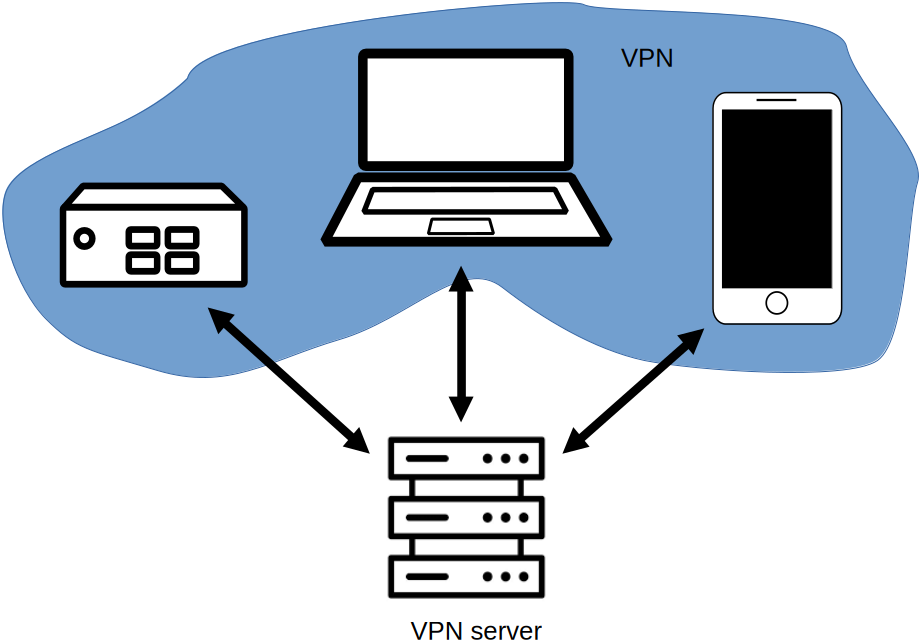
\includegraphics[width=.7\textwidth]{fig/vpn.png}
	\caption{The network architecture of the system}
	\label{fig-map}
\end{figure}

The PC runs Debian Linux 12.5 in headless mode, i.e. it is accessible
only through remote connections. Shell access is granted via
SSH (Secure Shell), providing command-line control. Since the signal
processing software (WSJT-X, discussed later) requires a graphical interface, a
VNC (Virtual Network Computing) \cite{richardson1998} session is configured to launch automatically
upon startup. This allows the desktop environment to be accessed remotely using
a VNC viewer, such as RealVNC, providing full graphical access to the system.

To provide more flexible remote access the PC is connected to a VPN (Virtual
Private Network) using OpenVPN. The OpenVPN client automatically connets to
the server during bootup and reconnects in case of any network error.

The decoding of the FT8 communication is done using WSJT-X.
WSJT-X (Weak Signal Joe Taylor - Extended) is an open-source software suite
specifically designed for weak-signal communication by amateur radio operators.
Developed by Nobel Prize-winning physicist Joe Taylor (K1JT) and a team of
contributors, WSJT-X supports various digital modes like FT8, JT65, JT9, and
WSPR, which are optimized for low-power, long-distance communication even under
challenging conditions. These modes are particularly useful when working with
faint or distorted signals, allowing users to make successful contacts in
situations where traditional voice or Morse code communication would fail. The
software uses advanced signal processing algorithms to decode transmissions at
or below the noise floor, making it highly effective for weak-signal work.

One of WSJT-X's most popular modes is FT8, which has gained widespread adoption
in the amateur radio community due to its efficiency and reliability. FT8, for
example, allows brief, structured exchanges in just 15-second transmission
intervals, making it ideal for quick and automated contacts across great
distances. WSJT-X provides a user-friendly graphical interface, real-time
decoding, and automated message exchanges, making it accessible to both
beginner and experienced operators. Additionally, it supports logging and
integration with other radio control software, further enhancing its
versatility. Overall, WSJT-X is a powerful tool for maximizing communication
possibilities under poor propagation or limited-power conditions.

WSJT-X generates several log files ALL.TXT containing all the decoded messages.

\cite{silver2011}
%ARRL handbook

\cite{cervera2021}
%Hullamterjedes, ionoszfera


\cite{hartje2020}
%Neumeyer III station, WSPR beacon. A hullamterjedest vizsgaljak vele, kifejezetten az antarktiszi kornyezetben

\cite{zolesi2014}
%Kulonbozo ionoszfera modellek, retegek, elorejelzes

\cite{taylor2010}
%Ez magarol a WSPR-rol szol

\cite{hunsucker2007}
%Ez is az ionoszferarol szol, konyv

\section{Results}

\subsection{Collected data and preprocessing}

The data collection system was continuously run for a year, from Jun 25 2024 to Jun 25 2025,
decoding ang logging 30,819,847 messages. Since the system was not equipped with an
uninterruptible power supply (UPS) unexpected power failures were occured, causing
minor errors in the ALL.txt log file.
Another source of errors is false decoding. Since FT8 is primarily designed for
human operation, WSJT-X is intentionally configured to be highly
permissive -- favoring the risk of false positives over missed valid decodes. In
typical usage, this trade-off is acceptable, as the software’s automatic
sequencing halts upon a false decode; a non-existent station will not respond,
preventing the exchange from continuing.

The processing algorithms filter messages based on the occurence of observed
callsign-grid square pairs: messages originating from sources that appear fewer
times than a configurable threshold are disregarded.

\subsection{Accessed grid squares}

\begin{figure*}[bt]
	\centering
	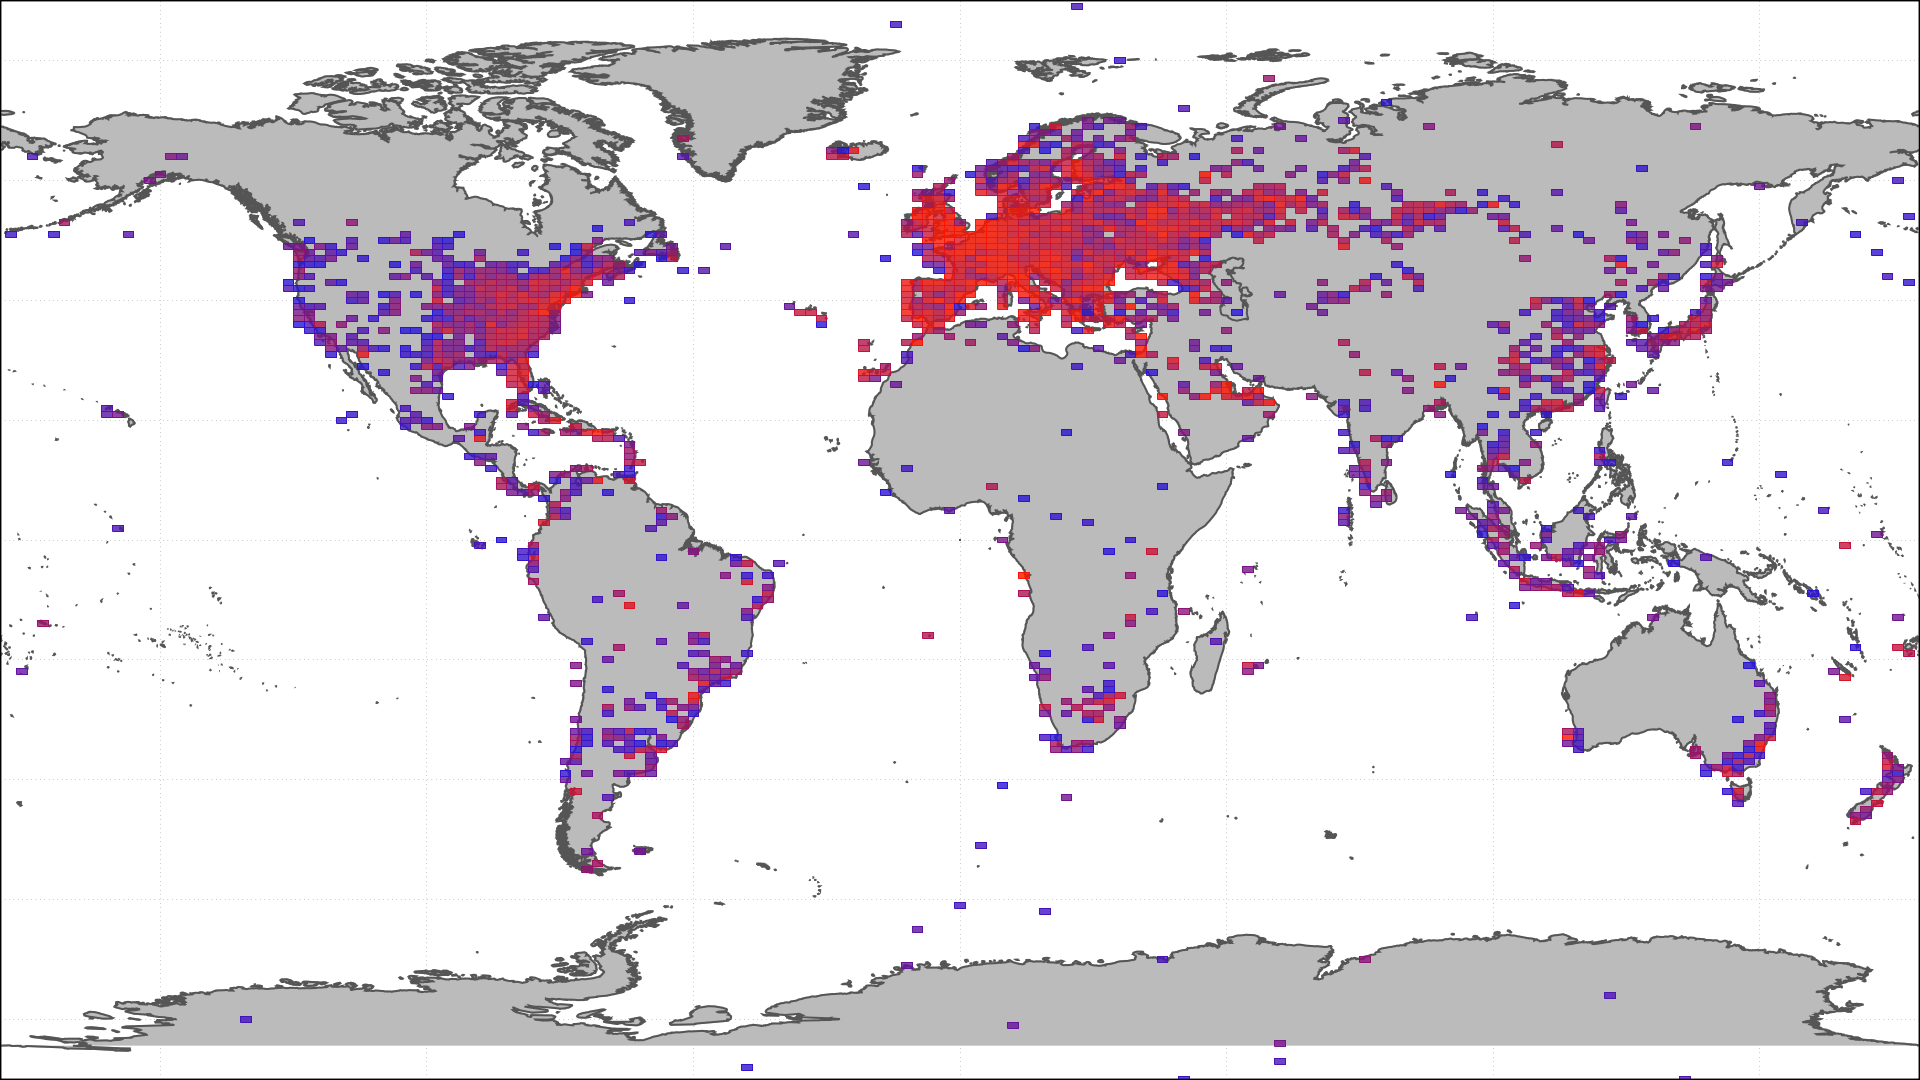
\includegraphics[width=1\textwidth]{fig/map.png}
	\caption{Map of 4-character Maidenhead grid squares, where CQ messages were received from.
  More red colors denote more active areas.}
	\label{fig-map}
\end{figure*}

To provide an overall view of the collected data, a heat map of grid squares
was generated, illustrating the spatial distribution and density of captured
messages across different geographical regions, as shown in Fig.~\ref{fig-map}.
Blue color means less captured messages, red color means more.

The map is clearly dominated by Europe and the eastern United States, both
forming large, continuous regions of activity. Additional areas with
significant coverage include Central America, Japan, the eastern and
southwestern coasts of Australia, New Zealand, and Indonesia. In contrast,
other regions exhibit only sporadic FT8 activity.

Numerous islands -- such as the Canary Islands, Cape Verde, St. Helena,
Seychelles, Mauritius, Réunion, and many smaller ones -- also display a high
density of contacts. This measurement is somewhat biased, as these locations
are popular among amateur radio operators who actively seek rare or remote
contacts.

An interesting phenomenon is the presence of signal sources in the open ocean,
which can be attributed to maritime vessels equipped with ham radio transceivers.

Lastly, Antarctica also appears on the map with notable FT8 activity,
particularly around the Neumayer Station III.




\section{Summary}


\bibliography{references}

\end{document}
